\section{Specifica componenti}

%diagramma del package%
\subsection{premi/server}
\begin{figure}[h]
\begin{center}
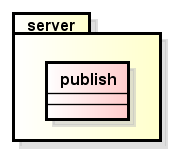
\includegraphics[scale=0.45]{img/diapkg/server.png}
\caption{Diagramma del package premi/client}
\end{center}
\end{figure}


%-------  diagramma della classe%
\subsubsection{premi/server/publish}
\begin{figure}[h]
\begin{center}
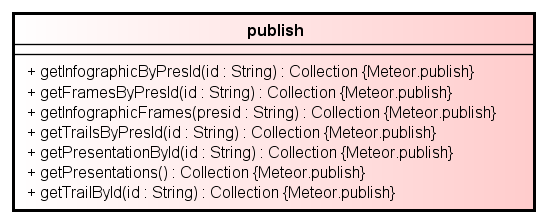
\includegraphics[scale=0.90]{img/diacla/publish.png}
\caption{Diagramma della classe premi/server/publish}
\end{center}
\end{figure}




\begin{description}
%-------  descrizione della classe%
\item[Descrizione] \hfill \\
	Lista di metodi che permettono al client di interagire con il database del server. I metodi marcati \texttt{[Meteor.methods]} devono essere inseriti nel servizio \$meteor per permettere poi al client di accedervi attraverso il pattern Dependency Injection$_G$, mentre quelli marcati \texttt{[Meteor.publish]} hanno lo scopo di pubblicare al client soltanto le informazioni a cui esso puo' accedere.
	
	
%-------  lista dei metodi%	
\item[Metodi] \hfill \\

	% -- inizio metodo -- %
	\begin{description}
		\item[\texttt{- removeFrameInf(idFrame : String, idInf : String, user : String) : void			}] \hfill \\
			Metodo privato di utilità che rimuove ogni occorrenza di un frame da un'infografica.
			
		\begin{description}
			% -- lista argomenti del metodo -- %
			\item[Argomenti] \hfill \\
				\begin{itemize}
				
					\item \texttt{idFrame : String			} \hfill \\
					Codice identificativo del frame da rimuovere
					\item \texttt{idInf : String		} \hfill \\
					Codice identificativo dell'infografica che possiede il frame
					\item \texttt{user : String			} \hfill \\
					Codice identificativo dell'utente che sta effettuando la rimozione
					
				\end{itemize}
			% -- note aggiuntive sul metodo -- %
			\item[Note] \hfill \\
			\begin{itemize}
					\item Il client non deve poter accedere direttamente a questo metodo
				\end{itemize}
		\end{description}
	\end{description}
	% -- fine metodo -- %	
	
	% -- inizio metodo -- %
	\begin{description}
		\item[\texttt{-removeFrameFromTrail(idFrame : String, idTrail : String, user :  String)	: void		}] \hfill \\
			Metodo privato di utilità che rimuove ogni occorrenza di un frame da un trail
			
		\begin{description}
			% -- lista argomenti del metodo -- %
			\item[Argomenti] \hfill \\
				\begin{itemize}
				
					\item \texttt{idFrame : String			} \hfill \\
					Codice identificativo del frame da rimuovere
					\item \texttt{idTrail : String			} \hfill \\
					Codice identificativo del trail che possiede il frame
					\item \texttt{user : String			} \hfill \\
					Codice identificativo dell'utente che sta effettuando la rimozione
					
				\end{itemize}
			% -- note aggiuntive sul metodo -- %
			\item[Note] \hfill \\
			\begin{itemize}
					\item Il client non deve poter accedere direttamente a questo metodo
				\end{itemize}
		\end{description}
	\end{description}
	% -- fine metodo -- %	

	% -- inizio metodo -- %
	\begin{description}
		\item[\texttt{+ CurrentUser() : Collection			}] \hfill \\
			Restituisce le informazioni riguardanti l'utente che sta interrogando il database attraverso una collezione di documenti di MongoDB
			
		\begin{description}
			
			% -- note aggiuntive sul metodo -- %
			\item[Note] \hfill \\
			\begin{itemize}
					\item Dev'essere inserito nel servizio \texttt{\$meteor} attraverso il comando Meteor.methods
				\end{itemize}
		\end{description}
	\end{description}
	% -- fine metodo -- %	

	% -- inizio metodo -- %
	\begin{description}
		\item[\texttt{+ insertPresentation(title : String, description : String) : String			}] \hfill \\
			Aggiunge una nuova presentazione nel database di proprietà dell'utente, e restituisce il suo codice identificativo
			
		\begin{description}
			% -- lista argomenti del metodo -- %
			\item[Argomenti] \hfill \\
				\begin{itemize}
				
					\item \texttt{title : String			} \hfill \\
					Titolo della nuova presentazione
					\item \texttt{description : String			} \hfill \\
					Descrizione della nuova presentazione
					
				\end{itemize}
			% -- note aggiuntive sul metodo -- %
			\item[Note] \hfill \\
			\begin{itemize}
					\item Dev'essere inserito nel servizio \texttt{\$meteor} attraverso il comando Meteor.methods
					\item Inizializzare ogni attributo della presentazione:
					\begin{itemize}
					\item \texttt{title} con il titolo ricevuto
					\item \texttt{description} con la descrizione ricevuta
					\item \texttt{owner} con l'id dell'utente che sta creando la presentazione
					\item \texttt{isPublic} : \texttt{false}, la presentazione inizialmente è sempre privata
					\end{itemize}
					\item Ogni presentazione possiede almeno un'infografica, che andrà creata e inizializata nel database con i seguenti campi dato:
					\begin{itemize}
					\item \texttt{dataX} -5000
					\item \texttt{dataY} -4000
					\item \texttt{dataZ} 0
					\item \texttt{scale} 0
					\item \texttt{height} 7920
					\item \texttt{width} 10240
					\item \texttt{zoom} 0
					\item \texttt{presid} il codice univoco della presentazione
					\item \texttt{owner} l'id dell'utente che sta creando la presentazione
					\item \texttt{background} Collezione(JSON) vuota
					\item \texttt{content} Collezione(JSON) vuota
					\item \texttt{framesId} array vuoto
					\item \texttt{type} "infographics"
					\end{itemize}
				\end{itemize}
		\end{description}
	\end{description}
	% -- fine metodo -- %	

	% -- inizio metodo -- %
	\begin{description}
		\item[\texttt{+ editPresentation(id : String, title : String, description : String) : void			}] \hfill \\
			Modifica le informazioni di una presentazione (titolo e descrizione)
			
		\begin{description}
			% -- lista argomenti del metodo -- %
			\item[Argomenti] \hfill \\
				\begin{itemize}
				
					\item \texttt{title : String			} \hfill \\
					Nuovo titolo della presentazione
					\item \texttt{description : String			} \hfill \\
					Nuova descrizione della presentazione
					
				\end{itemize}
			% -- note aggiuntive sul metodo -- %
			\item[Note] \hfill \\
			\begin{itemize}
					\item Dev'essere inserito nel servizio \texttt{\$meteor} attraverso il comando Meteor.methods
				\end{itemize}
		\end{description}
	\end{description}
	% -- fine metodo -- %	

	% -- inizio metodo -- %
	\begin{description}
		\item[\texttt{+ publicPresentation(id : String, pub : boolean) : void			}] \hfill \\
			Rende una presentazione pubblica o privata
			
		\begin{description}
			% -- lista argomenti del metodo -- %
			\item[Argomenti] \hfill \\
				\begin{itemize}
				
					\item \texttt{id :  String			} \hfill \\
					Codice identificativo della presentazione
					\item \texttt{pub :  boolean			} \hfill \\
					Indica se la presentazione è pubblica (\texttt{true}) o privata (\texttt{false})
					
				\end{itemize}
			% -- note aggiuntive sul metodo -- %
			\item[Note] \hfill \\
			\begin{itemize}
					\item Dev'essere inserito nel servizio \texttt{\$meteor} attraverso il comando Meteor.methods
				\end{itemize}
		\end{description}
	\end{description}
	% -- fine metodo -- %	
	
	% -- inizio metodo -- %
	\begin{description}
		\item[\texttt{+ removePresentation(id : String) : boolean			}] \hfill \\
			Rimuove una presentazione dal database. Restituisce un valore che indica se l'operazione è avvenuta con successo
			
		\begin{description}
			% -- lista argomenti del metodo -- %
			\item[Argomenti] \hfill \\
				\begin{itemize}
				
					\item \texttt{id : String			} \hfill \\
					Codice identificativo della presentazione.
					
				\end{itemize}
			% -- note aggiuntive sul metodo -- %
			\item[Note] \hfill \\
			\begin{itemize}
					\item Devono essere rimossi, assieme alla presentazione, anche tutti gli altri dati ad essa associati (frame, infografica e trails)
					\item Dev'essere inserito nel servizio \texttt{\$meteor} attraverso il comando Meteor.methods
				\end{itemize}
		\end{description}
	\end{description}
	% -- fine metodo -- %	
	
	% -- inizio metodo -- %
	\begin{description}
		\item[\texttt{+ getTrailById(id : String) : Collection			}] \hfill \\
			Restituisce il trail corrispondente al codice identificativo fornito, attraverso una collezione di documenti di MongoDB
			
		\begin{description}
			% -- lista argomenti del metodo -- %
			\item[Argomenti] \hfill \\
				\begin{itemize}
				
					\item \texttt{id : String			} \hfill \\
					Codice identificativo del trail che si sta cercando
					
				\end{itemize}
			% -- note aggiuntive sul metodo -- %
			\item[Note] \hfill \\
			\begin{itemize}
					\item Dev'essere inserito nel servizio \texttt{\$meteor} attraverso il comando Meteor.methods
				\end{itemize}
		\end{description}
	\end{description}
	% -- fine metodo -- %	
	
	% -- inizio metodo -- %
	\begin{description}
		\item[\texttt{+ insertTrail(title : String, presid : String) : void			}] \hfill \\
			Inserisce un nuovo trail associato ad una presentazione all'interno del database
			
		\begin{description}
			% -- lista argomenti del metodo -- %
			\item[Argomenti] \hfill \\
				\begin{itemize}
				
					\item \texttt{title : String			} \hfill \\
					Titolo del nuovo trail
					\item \texttt{presid : String			} \hfill \\
					Codice identificativo della presentazione a cui il trail è associato
					
				\end{itemize}
			% -- note aggiuntive sul metodo -- %
			\item[Note] \hfill \\
			\begin{itemize}
					\item Dev'essere inserito nel servizio \texttt{\$meteor} attraverso il comando Meteor.methods
					\item inizializzare il trail con i seguenti campi:
					\begin{itemize}
					\item \texttt{title} con il titolo ricevuto
					\item \texttt{owner} con l'id dell'utente che sta chiamando il metodo
					\item \texttt{presid} con il codice identificativo della presentazione
					\item \texttt{trail} è una matrice vuota ( \texttt{[[]]} )
					\end{itemize}
				\end{itemize}
		\end{description}
	\end{description}
	% -- fine metodo -- %	
	
	% -- inizio metodo -- %
	\begin{description}
		\item[\texttt{+ updateTrail(idTrail : int, update : Collection) : void			}] \hfill \\
			Aggiorna i dati di un trail con quelli forniti
			
		\begin{description}
			% -- lista argomenti del metodo -- %
			\item[Argomenti] \hfill \\
				\begin{itemize}
				
					\item \texttt{idTrail : String		} \hfill \\
					Codice identificativo del trail
					\item \texttt{update : Collection		} \hfill \\
					Insieme dei dati del trail modificati dall'utente
					
				\end{itemize}
			% -- note aggiuntive sul metodo -- %
			\item[Note] \hfill \\
			\begin{itemize}
					\item Dev'essere inserito nel servizio \texttt{\$meteor} attraverso il comando Meteor.methods
				\end{itemize}
		\end{description}
	\end{description}
	% -- fine metodo -- %		
	
	% -- inizio metodo -- %
	\begin{description}
		\item[\texttt{+ removeTrailById(id : String) : boolean			}] \hfill \\
			Rimuove dal database il trail associato al codice identificativo fornito. Restituisce \texttt{true} se l'operazione ha avuto successo, \texttt{false} altrimenti.
			
		\begin{description}
			% -- lista argomenti del metodo -- %
			\item[Argomenti] \hfill \\
				\begin{itemize}
				
					\item \texttt{id : String		} \hfill \\
					Codice identificativo del trail da rimuovere
					
				\end{itemize}
			% -- note aggiuntive sul metodo -- %
			\item[Note] \hfill \\
			\begin{itemize}
					\item Dev'essere inserito nel servizio \texttt{\$meteor} attraverso il comando Meteor.methods
				\end{itemize}
		\end{description}
	\end{description}
	% -- fine metodo -- %
	
	% -- inizio metodo -- %
	\begin{description}
		\item[\texttt{+ removeTrailsByIdPres(id : String) : void			}] \hfill \\
			Rimuove dal database ogni trail associato ad una presentazione
			
		\begin{description}
			% -- lista argomenti del metodo -- %
			\item[Argomenti] \hfill \\
				\begin{itemize}
				
					\item \texttt{id :  String		} \hfill \\
					Codice identificativo della presentazione da cui rimuovere ogni trail
					
				\end{itemize}
			% -- note aggiuntive sul metodo -- %
			\item[Note] \hfill \\
			\begin{itemize}
					\item Dev'essere inserito nel servizio \texttt{\$meteor} attraverso il comando Meteor.methods
				\end{itemize}
		\end{description}
	\end{description}
	% -- fine metodo -- %
	
	% -- inizio metodo -- %
	\begin{description}
		\item[\texttt{+ editTrailById(id : String, title : String) : void			}] \hfill \\
			Permette all'utente di rinominare un trail in suo possesso
			
		\begin{description}
			% -- lista argomenti del metodo -- %
			\item[Argomenti] \hfill \\
				\begin{itemize}
				
					\item \texttt{id : String		} \hfill \\
					Codice identificativo del trail da rinominare
					\item \texttt{title : String		} \hfill \\
					Nuovo titolo, o nome, del trail
					
				\end{itemize}
			% -- note aggiuntive sul metodo -- %
			\item[Note] \hfill \\
			\begin{itemize}
					\item Dev'essere inserito nel servizio \texttt{\$meteor} attraverso il comando Meteor.methods
				\end{itemize}
		\end{description}
	\end{description}
	% -- fine metodo -- %
	
	% -- inizio metodo -- %
	\begin{description}
		\item[\texttt{+ insertFrameByIdPres(presid : String) : String			}] \hfill \\
			Inserisce un nuovo frame all'interno di una presentazione, e restituisce il suo id
			
		\begin{description}
			% -- lista argomenti del metodo -- %
			\item[Argomenti] \hfill \\
				\begin{itemize}
				
					\item \texttt{presid : String			} \hfill \\
					Codice identificativo della presentazione a cui assegnare il nuovo frame
					
				\end{itemize}
			% -- note aggiuntive sul metodo -- %
			\item[Note] \hfill \\
			\begin{itemize}
					\item Dev'essere inserito nel servizio \texttt{\$meteor} attraverso il comando Meteor.methods
					\item Inizializzare il frame con i seguenti campi dato:
					\begin{itemize}
					\item \texttt{presid} con il codice identificativo della presentazione
					\item \texttt{owner} con l'id dell'utente che ha effetuato la chiamata al metodo
					\item \texttt{dataX} 0
					\item \texttt{dataY} 0
					\item \texttt{dataZ} 0
					\item \texttt{height} 792
					\item \texttt{width} 1024
					\item \texttt{scale} 1
					\item \texttt{backgroundColor} "#FFFFFF"
					\item \texttt{content} Collezione(JSON) vuota
					\item \texttt{type} frame
					\item \texttt{lvl} 0
					\end{itemize}
				\end{itemize}
		\end{description}
	\end{description}
	% -- fine metodo -- %
	
	% -- inizio metodo -- %
	\begin{description}
		\item[\texttt{+ editFrameById(idframe : String, update : Collection) : void			}] \hfill \\
			Modifica un frame con nuovi dati inseriti dall'utente
			
		\begin{description}
			% -- lista argomenti del metodo -- %
			\item[Argomenti] \hfill \\
				\begin{itemize}
				
					\item \texttt{idframe : String			} \hfill \\
					Codice identificativo del frame
					\item \texttt{update : Collection		} \hfill \\
					Collezione di dati modificati del frame da salvare sul database
					
				\end{itemize}
			% -- note aggiuntive sul metodo -- %
			\item[Note] \hfill \\
			\begin{itemize}
					\item Dev'essere inserito nel servizio \texttt{\$meteor} attraverso il comando Meteor.methods
				\end{itemize}
		\end{description}
	\end{description}
	% -- fine metodo -- %
	
	% -- inizio metodo -- %
	\begin{description}
		\item[\texttt{removeFrameById(id : String) : void			}] \hfill \\
			Rimuove dal database il frame corrispondente al codice identificativo inviato
			
		\begin{description}
			% -- lista argomenti del metodo -- %
			\item[Argomenti] \hfill \\
				\begin{itemize}
				
					\item \texttt{id : String			} \hfill \\
					Codice identificativo del frame da rimuovere
					
				\end{itemize}
			% -- note aggiuntive sul metodo -- %
			\item[Note] \hfill \\
			\begin{itemize}
					\item Dev'essere inserito nel servizio \texttt{\$meteor} attraverso il comando Meteor.methods
					\item Il frame dev'essere rimosso anche dai trail e dalle infografiche in cui è stato utilizzato. Servirsi dei metodi removeFrameFromTrail e RemoveFramInf
				\end{itemize}
		\end{description}
	\end{description}
	% -- fine metodo -- %
	
	% -- inizio metodo -- %
	\begin{description}
		\item[\texttt{+ removeFramesByIdPres(id : String) : void			}] \hfill \\
			Rimuove dal database tutti i frame associati ad una presentazione.
			
		\begin{description}
			% -- lista argomenti del metodo -- %
			\item[Argomenti] \hfill \\
				\begin{itemize}
				
					\item \texttt{id : String			} \hfill \\
					Codice identificativo della presentazione
					
				\end{itemize}
			% -- note aggiuntive sul metodo -- %
			\item[Note] \hfill \\
			\begin{itemize}
					\item Dev'essere inserito nel servizio \texttt{\$meteor} attraverso il comando Meteor.methods
				\end{itemize}
		\end{description}
	\end{description}
	% -- fine metodo -- %
	
	% -- inizio metodo -- %
	\begin{description}
		\item[\texttt{+  insertInfographicByIdPres(presid : String) : String			}] \hfill \\
			Inserisce un'infografica nel database associandola ad una presentazione, e restituisce il suo codice identificativo
			
		\begin{description}
			% -- lista argomenti del metodo -- %
			\item[Argomenti] \hfill \\
				\begin{itemize}
				
					\item \texttt{presid : String			} \hfill \\
					Codice identificativo della presentazione
					
				\end{itemize}
			% -- note aggiuntive sul metodo -- %
			\item[Note] \hfill \\
			\begin{itemize}
					\item Dev'essere inserito nel servizio \texttt{\$meteor} attraverso il comando Meteor.methods
					\item L'Infografica dev'essere inizializzata con i seguenti campi dato:
					\begin{itemize}
					\item \texttt{presid} il codice identificativo della presentazione
					\item \texttt{owner} Il codice identificativo dell'utente che ha chiamato il metodo
					\item \texttt{content} Collezione(JSON) vuota
					\item \texttt{frames} Collezione(JSON) vuota
					\item \texttt{type} "infographic"
					\end{itemize}
				\end{itemize}
		\end{description}
	\end{description}
	% -- fine metodo -- %
	
	% -- inizio metodo -- %
	\begin{description}
		\item[\texttt{+ updateInfographicById(idInf : String, update : Collection) : void			}] \hfill \\
			Aggiorna un'infografica con campi dati modificati dall'utente
			
		\begin{description}
			% -- lista argomenti del metodo -- %
			\item[Argomenti] \hfill \\
				\begin{itemize}
				
					\item \texttt{idInf : String			} \hfill \\
					Codice identificativo dell'infografica da aggiornare
					\item \texttt{update : Collection			} \hfill \\
					Collezione di dati con cui aggiornare l'infografica
					
				\end{itemize}
			% -- note aggiuntive sul metodo -- %
			\item[Note] \hfill \\
			\begin{itemize}
					\item Dev'essere inserito nel servizio \texttt{\$meteor} attraverso il comando Meteor.methods
				\end{itemize}
		\end{description}
	\end{description}
	% -- fine metodo -- %\\
	
	% -- inizio metodo -- %
	\begin{description}
		\item[\texttt{+ updateGOContentFrame(idGO : String, update : Collection, idFrame : String) : void			}] \hfill \\
			Aggiorna un oggetto grafico contenuto all'interno di una presentazione con  campi dati modificati dall'utente
			
		\begin{description}
			% -- lista argomenti del metodo -- %
			\item[Argomenti] \hfill \\
				\begin{itemize}
				
					\item \texttt{idGO : String			} \hfill \\
					Codice identificativo del Frame da modificare
					
				\end{itemize}
			% -- note aggiuntive sul metodo -- %
			\item[Note] \hfill \\
			\begin{itemize}
					\item Deve essere esplicitamente marcato come costante (?)
					\item Deve possedere qualche caratteristica
					\item Metodo ridefinito
				\end{itemize}
		\end{description}
	\end{description}
	% -- fine metodo -- %
	
	% -- inizio metodo -- %
	\begin{description}
		\item[\texttt{+ void operation0()			}] \hfill \\
			Descrizione del metodo
			
		\begin{description}
			% -- lista argomenti del metodo -- %
			\item[Argomenti] \hfill \\
				\begin{itemize}
				
					\item \texttt{nomeArgomento : tipoArgomento			} \hfill \\
					Descrizione argomento
					
				\end{itemize}
			% -- note aggiuntive sul metodo -- %
			\item[Note] \hfill \\
			\begin{itemize}
					\item Deve essere esplicitamente marcato come costante (?)
					\item Deve possedere qualche caratteristica
					\item Metodo ridefinito
				\end{itemize}
		\end{description}
	\end{description}
	% -- fine metodo -- %
	
	
	
	
\end{description}